
\chapter{VAR Models Under Non-Normal Errors}

In practice, the assumption of normality in errors is not often satisfied.
Simply put, the normal distribution doesn't adequately describe much
\textquotedbl{}real world\textquotedbl{}\ data. This is sometimes
remedied through arbitrary transformations to achieve near-normality,
however, that should not be the goal. \ It doesn't make sense to
manipulate data to fit a model any more than it makes sense to put
a square peg into a round hole. The goal of modeling should be to
fit the best model possible to the data, not the other way around.
To this end, models based on more general distributions are required.
There are many more robust and adaptive choices to model the distribution
of the errors such as the Multivariate Pearson Family of distributions,
the Multivariate Power Exponential (PE) Distribution \citet{Gome:Gome:Mari:1998},
and the Multivariate Generalized t Distribution (MGT) \citet{Arsl:2004}\ to
name a few.


\section{Power Exponential Errors}

One possible choice for a more adaptive and robust error term is the
Multivariate Power Exponential (PE) Distribution \citet{Gome:Gome:Mari:1998}.
For the multivariate regression model, this has been initially explored
\citet{Liu:Boz:2004}. Here it is adapted to the VAR framework, which
can be written in the multivariate regression format, as seen in (\ref{VAR (Matrix)}),
(\ref{VAR (Vec)}), and (\ref{Subset VAR (Vec)}).

The univariate PE distribution was initially introduced, as an extension
to the normal distribution, by \citet{Subb:1923}, and has been used
by \citet{Box:1953} and \citet{Box:Tiao:1973}. The univariate PE
distribution is defined as
\begin{equation}
f\left(x;\mu,\sigma,\beta\right)=\frac{1}{\sigma\Gamma\left(1+\frac{1}{2\beta}\right)2^{1+\frac{1}{2\beta}}}\exp\left(-\frac{1}{2}\left\vert \frac{x-\mu}{\sigma}\right\vert ^{2\beta}\right),\label{Univariate PE}
\end{equation}
where $\mu\in\mathbb{R}$ is the location, $\sigma>0$ is the scale,
and $\beta>0$ is the shape parameter which is related to kurtosis.
The PE distribution is robust in that (\ref{Univariate PE}) can represent
many symmetric unimodal distributions. When $\beta=1$ (\ref{Univariate PE})
is the Normal distribution, for $\beta=.5$ it is the Laplace, or
Double Exponential distribution, and as $\beta\rightarrow\infty$
(\ref{Univariate PE}) becomes the Uniform distribution.

\citet{Gome:Gome:Mari:1998} develop a multivariate generalization
of the univariate PE, denoted $PE_{k}\left(\mathbf{\mu},\Sigma,\beta\right)$,
defined as
\begin{equation}
f\left(\mathbf{x};\mathbf{\mu},\Sigma,\beta\right)=C\left\vert \Sigma\right\vert ^{-\frac{1}{2}}\exp\left(-\frac{1}{2}\left[\left(\mathbf{x}-\mathbf{\mu}\right)^{\prime}\Sigma^{-1}\left(\mathbf{x}-\mathbf{\mu}\right)\right]^{\beta}\right),\label{Multivariate PE}
\end{equation}
where
\[
C=\frac{k\Gamma\left(\frac{k}{2}\right)}{\pi^{\frac{k}{2}}\Gamma\left(1+\frac{k}{2\beta}\right)2^{1+\frac{k}{2\beta}}},
\]
and $\mu\in\mathbb{R}^{k}$ is the location, $\Sigma$ is the $\left(k\times k\right)$
positive definite scale matrix, and $\beta>0$ is the shape parameter
which is related to kurtosis. This formulation is particularly attractive
given that when $k=1$, (\ref{Multivariate PE}) reduces to (\ref{Univariate PE}).
Figure \ref{PE Distribution Plots} shows the shape of a bivariate
power exponential for various choices of $\beta$. To be useful for
time series, a further modification is necessary. This is where the
matrix variate power exponential distribution, denoted $MPE_{n\times k}\left(\mathbf{\mu},\Phi,\Sigma,\beta\right)$
and developed by \citet{Sanch:Gome:Mari:2002}, becomes useful.

Here we make the assumption that the errors are distributed as multivariate
power exponential, that is
\[
\mathbf{\varepsilon}\thicksim PE_{nk}\left(\mathbf{0},\Omega,\beta\right),
\]
where $\Omega=\Sigma\otimes\mathbf{I}_{n}$. Therefore, the probability
density function (pdf) of $\mathbf{\varepsilon}$\ is
\begin{eqnarray*}
f\left(\mathbf{\varepsilon}\right) & = & \frac{nk\Gamma\left(\frac{nk}{2}\right)}{\pi^{\frac{nk}{2}}\Gamma\left(1+\frac{nk}{2\beta}\right)2^{1+\frac{nk}{2\beta}}}\left\vert \Omega\right\vert ^{-\frac{1}{2}}\exp\left(-\frac{1}{2}\left[\mathbf{\varepsilon}^{\prime}\Omega^{-1}\mathbf{\varepsilon}\right]^{\beta}\right)\\
 & = & \frac{nk\Gamma\left(\frac{nk}{2}\right)}{\pi^{\frac{nk}{2}}\Gamma\left(1+\frac{nk}{2\beta}\right)2^{1+\frac{nk}{2\beta}}}\left\vert \Sigma\otimes\mathbf{I}_{n}\right\vert ^{-\frac{n}{2}}\exp\left(-\frac{1}{2}\left[\left(\mathbf{y}-\mathbf{x}^{\ast}\mathbf{\gamma}\right)^{\prime}\left(\Sigma^{-1}\otimes\mathbf{I}_{n}\right)\left(\mathbf{y}-\mathbf{x}^{\ast}\mathbf{\gamma}\right)\right]^{\beta}\right)
\end{eqnarray*}


\begin{eqnarray*}
l\left(\theta\right) & \equiv & \log L\left(\theta\right)=\log\left(nk\Gamma\left(\frac{nk}{2}\right)\right)-\frac{nk}{2}\log\left(\pi\right)\\
 &  & -\log\Gamma\left(1+\frac{nk}{2\beta}\right)-\left(1+\frac{nk}{2\beta}\right)\log\left(2\right)\\
 &  & -\frac{n}{2}\log\left\vert \Sigma^{-1}\otimes\mathbf{I}_{n}\right\vert -\frac{1}{2}\left[\left(\mathbf{y}-\mathbf{x\beta}\right)^{\prime}\left(\Sigma^{-1}\otimes\mathbf{I}_{n}\right)\left(\mathbf{y}-\mathbf{x\beta}\right)\right]^{\beta}
\end{eqnarray*}


\[
\frac{\partial l\left(\theta\right)}{\partial\mathbf{\beta}}=\beta\mathbf{x}^{\prime}\left(\Sigma^{-1}\otimes\mathbf{I}_{n}\right)\left(\mathbf{y}-\mathbf{x\beta}\right)\left[\left(\mathbf{y}-\mathbf{x\beta}\right)^{\prime}\left(\Sigma^{-1}\otimes\mathbf{I}_{n}\right)\left(\mathbf{y}-\mathbf{x\beta}\right)\right]^{\beta-1}
\]


\[
\frac{\partial l\left(\theta\right)}{\partial\mathbf{\beta}}
\]
\[
f\left(\mathbf{\varepsilon}\right)=\frac{nk\Gamma\left(\frac{nk}{2}\right)}{\pi^{\frac{nk}{2}}\Gamma\left(1+\frac{nk}{2\beta}\right)2^{1+\frac{nk}{2\beta}}}\left\vert \Sigma\right\vert ^{-\frac{n}{2}}\exp\left(-\frac{1}{2}tr\left[\Sigma^{-1}\left(\mathbf{Y}-\mathbf{XB}\right)^{\prime}\left(\mathbf{Y}-\mathbf{XB}\right)\right]^{\beta}\right)
\]


\begin{figure}[ptb]
\begin{centering}
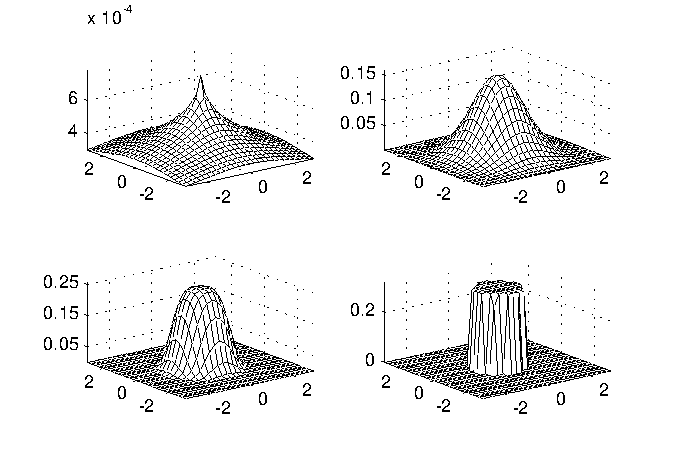
\includegraphics[bb=0bp 0bp 4.4987000000000004in 2.9922in,width=4.5515in,height=3.0364in,bb = 0 0 200 100, draft, type=eps]{F:/Personal/Dissertation/Lyx/figures/pdf/PE_Dist_Plots__1.pdf}\caption{$PE_{2}\left(\mathbf{\mu},\Sigma,\beta\right)$ density plots with
$\mathbf{\mu}=\left[0,0\right]^{\prime}$ and $\Sigma=I_{2}$ for
various choices of $\beta$.}

\par\end{centering}

\centering{}\label{PE Distribution Plots}
\end{figure}



\subsection{Model Selection}

Using the results from (\ref{Normal logLikelihood}), the Information
Criteria can be calculated.


\subsubsection{AIC}

\begin{eqnarray*}
AIC\left(m\right) & = & -2\log L\left(\widetilde{\theta}_{m}\right)+2r_{m}\\
 & = & nk\log\left(2\pi\right)+n\log\left\vert \widetilde{\Sigma}_{m}\right\vert +nk\\
 &  & +2\left(l_{m}+k\left(k+1\right)/2\right).
\end{eqnarray*}



\subsubsection{SBC}

\begin{eqnarray*}
SBC\left(m\right) & = & -2\log L\left(\widetilde{\theta}_{m}\right)+r_{m}\log\left(n\right)\\
 & = & nk\log\left(2\pi\right)+n\log\left\vert \widetilde{\Sigma}_{m}\right\vert +nk\\
 &  & +\left(l_{m}+k\left(k+1\right)/2\right)\log\left(n\right).
\end{eqnarray*}



\subsubsection{HQ}

\begin{eqnarray*}
HQ\left(m\right) & = & -2\log L\left(\widetilde{\theta}_{m}\right)+r_{m}\log\log\left(n\right)\\
 & = & nk\log\left(2\pi\right)+n\log\left\vert \widetilde{\Sigma}_{m}\right\vert +nk\\
 &  & +\left(l_{m}+k\left(k+1\right)/2\right)\log\log\left(n\right).
\end{eqnarray*}



\subsubsection{AIC$_{\text{C}}$}

\begin{eqnarray*}
AIC_{C_{A}}\left(m\right) & = & -2\log L\left(\widetilde{\theta}_{m}\right)+2\frac{r_{m}}{n-r_{m}-1}\\
 & = & nk\log\left(2\pi\right)+n\log\left\vert \widetilde{\Sigma}_{m}\right\vert +nk\\
 &  & +2\frac{\left(l_{m}+k\left(k+1\right)/2\right)}{n-\left(l_{m}+k\left(k+1\right)/2\right)-1}
\end{eqnarray*}


\begin{eqnarray*}
AIC_{C_{B}}\left(m\right) & = & -2\log L\left(\widetilde{\theta}_{m}\right)+2\frac{r_{m}}{n-r_{m}-(k+1)/2}\\
 & = & nk\log\left(2\pi\right)+n\log\left\vert \widetilde{\Sigma}_{m}\right\vert +nk\\
 &  & +2\frac{\left(l_{m}+k\left(k+1\right)/2\right)}{n-\left(l_{m}+k\left(k+1\right)/2\right)-\left(k+1\right)/2}
\end{eqnarray*}



\subsubsection{CAIC}

\begin{eqnarray*}
CAIC\left(m\right) & = & -2\log L\left(\widetilde{\theta}_{m}\right)+r_{m}\left(\log\left(n\right)+1\right)\\
 & = & nk\log\left(2\pi\right)+n\log\left\vert \widetilde{\Sigma}_{m}\right\vert +nk\\
 &  & +\left(l_{m}+k\left(k+1\right)/2\right)\left(\log\left(n\right)+1\right)
\end{eqnarray*}



\subsubsection{CAICF}

\begin{eqnarray*}
CAICF\left(m\right) & = & -2\log L\left(\widetilde{\theta}_{m}\right)+r_{m}\left[\log n+2\right]+\log\left\vert \hat{\mathcal{F}}^{-1}\right\vert \\
 & = & nk\log\left(2\pi\right)+n\log\left\vert \widetilde{\Sigma}_{m}\right\vert +nk\\
 &  & +\left(l_{m}+k\left(k+1\right)/2\right)\left(\log\left(n\right)+2\right)+\log\left\vert \hat{\mathcal{F}}^{-1}\right\vert 
\end{eqnarray*}



\subsubsection{CAICF$_{\text{E}}$}

\begin{eqnarray*}
CAICF_{E}\left(m\right) & = & -2\log L\left(\widetilde{\theta}_{m}\right)+r_{m}\left[\log n+2\right]+\log\left\vert \hat{\mathcal{F}}^{-1}\right\vert \\
 &  & +2tr\left(\hat{\mathcal{F}}^{-1}\hat{R}\right)\\
 & = & nk\log\left(2\pi\right)+n\log\left\vert \widetilde{\Sigma}_{m}\right\vert +nk\\
 &  & +\left(l_{m}+k\left(k+1\right)/2\right)\left(\log\left(n\right)+2\right)+\log\left\vert \hat{\mathcal{F}}^{-1}\right\vert \\
 &  & +2tr\left(\hat{\mathcal{F}}^{-1}\hat{R}\right)
\end{eqnarray*}



\subsubsection{CAICF$_{\text{C}}$}

\begin{eqnarray*}
CAICF_{C}\left(m\right) & = & -2\log L\left(\widetilde{\theta}_{m}\right)+r_{m}\left[\log n+2\right]+\log\left\vert \hat{\mathcal{F}}^{-1}\right\vert \\
 &  & +2\left(\frac{nr_{m}}{n-r_{m}-2}\right)\\
 & = & nk\log\left(2\pi\right)+n\log\left\vert \widetilde{\Sigma}_{m}\right\vert +nk\\
 &  & +\left(l_{m}+k\left(k+1\right)/2\right)\left(\log\left(n\right)+2\right)+\log\left\vert \hat{\mathcal{F}}^{-1}\right\vert \\
 &  & +2\left(\frac{nr_{m}}{n-r_{m}-2}\right)
\end{eqnarray*}



\subsubsection{GAIC}

\begin{eqnarray*}
GAIC\left(m\right) & = & -2\log L\left(\widetilde{\theta}_{m}\right)+2tr\left(\hat{\mathcal{F}}^{-1}\hat{R}\right)\\
 & = & nk\log\left(2\pi\right)+n\log\left\vert \widetilde{\Sigma}_{m}\right\vert +nk\\
 &  & +2tr\left(\hat{\mathcal{F}}^{-1}\hat{R}\right)
\end{eqnarray*}



\subsubsection{ICOMP}

\[
ICOMP\left(m\right)=-2\log L\left(\widetilde{\theta}_{m}\right)+2C_{1}\left(\hat{\mathcal{F}}^{-1}\left(\widetilde{\theta}_{m}\right)\right),
\]
where
\[
\hat{\mathcal{F}}^{-1}\left(\widetilde{\theta}_{m}\right)=\left[\begin{array}{cc}
\widehat{\mathbf{cov}}\left(\widetilde{\mathbf{\gamma}}_{m}\right) & \mathbf{0}\\
\mathbf{0} & \frac{2}{n}\mathbf{D}_{p}^{+}\left(\widetilde{\Sigma}_{m}\otimes\widetilde{\Sigma}_{m}\right)\mathbf{D}_{p}^{+\prime}
\end{array}\right],
\]
and $\widehat{\mathbf{cov}}\left(\widetilde{\mathbf{\gamma}}_{m}\right)$
is a consistent estimator of the asymptotic covariance matrix of the
subset VAR coefficients. \citet{Bea:Boz:1998} show that ICOMP can
be expressed as
\begin{eqnarray*}
ICOMP\left(m\right) & = & nk\left(\log\left(2\pi\right)+1\right)+n\log\left\vert \widetilde{\Sigma}_{m}\right\vert \\
 &  & +r_{m}\log\left(\frac{tr\left(\widehat{\mathbf{cov}}\left(\widetilde{\mathbf{\gamma}}_{m}\right)\right)+\frac{1}{2n}G_{m}}{r_{m}}\right)\\
 &  & -\log\left\vert \widehat{\mathbf{cov}}\left(\widetilde{\mathbf{\gamma}}_{m}\right)\right\vert -k\log\left(2\right)+\frac{k\left(k+1\right)}{2}\log\left(n\right)\\
 &  & -\left(k+1\right)\log\left\vert \widetilde{\Sigma}_{m}\right\vert 
\end{eqnarray*}
where
\[
G_{m}\equiv tr\left(\widetilde{\Sigma}_{m}^{2}\right)+\left(tr\left(\widetilde{\Sigma}_{m}\right)\right)^{2}+2\sum_{i=1}^{k}\widetilde{\sigma}_{i,m}^{2}
\]
and $\widetilde{\sigma}_{i,m}^{2}$ is the $i^{\text{th}}$ diagonal
element of $\widetilde{\Sigma}_{m}$.


\subsubsection{BMS}

\begin{eqnarray*}
BMS\left(m\right) & = & -2\log L\left(\widetilde{\theta}_{m}\right)+r_{m}\log n+\log\left\vert \hat{\mathcal{F}}^{-1}\right\vert +2tr\left(\hat{\mathcal{F}}^{-1}\hat{R}\right)\\
 & = & nk\log\left(2\pi\right)+n\log\left\vert \widetilde{\Sigma}_{m}\right\vert +nk\\
 &  & +\left(l_{m}+k\left(k+1\right)/2\right)\log n\\
 &  & +\log\left\vert \hat{\mathcal{F}}^{-1}\right\vert +2tr\left(\hat{\mathcal{F}}^{-1}\hat{R}\right)
\end{eqnarray*}



\section{Multivariate Generalized t Errors}

Another choice for a more adaptive and robust error term, along the
same lines of the Multivariate PE distribution, is the Multivariate
Generalized t Distribution (MGT) \citet{Arsl:2004}. Here, the VAR
model with MGT errors is developed.
